\section{The device}
The device is based upon a NodeMCU wi-fi board \footnote{This choice has been guided exlusively by the smaller dimension and cost of this board; an Arduino board with an appropriate wi-fi shield can of course do as well.}: sensors to measure weight, temperature and humidity are used, which will be described in the following; see last chapters to see some further implementations of a battery-level monitor and a resting capability.

\begin{figure} 
  \centering
  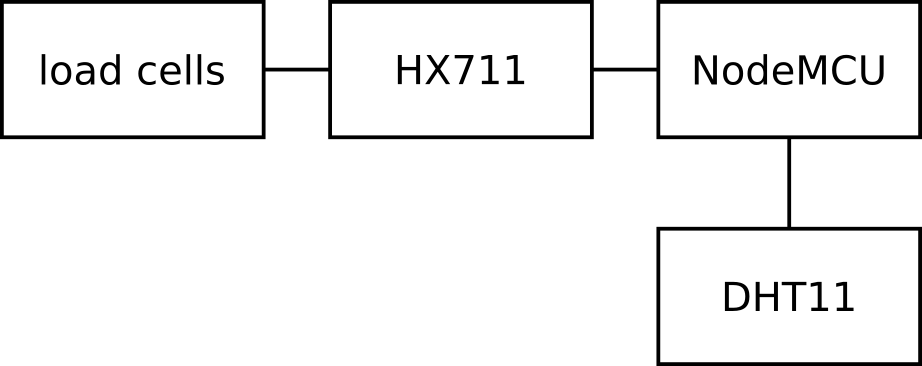
\includegraphics[width=0.7\textwidth]{latex/img/device_scheme.png}
  \caption{General scheme of the device.}\label{img:loadcells_scheme}
\end{figure}

\subsection{NodeMCU}
Programming the NodeMCU is as easy as writing Arduino code, provided that the support for Esp8266 is installed and the appropriate board is selected \footnote{\url{https://www.instructables.com/id/Quick-Start-to-Nodemcu-ESP8266-on-Arduino-IDE/}}.

\subsection{Weight - load cells + HX711}
A Wheatstone bridge configuration for four load cells is used \footnote{\url{https://www.aliexpress.com/item/1PCS-DIY-50Kg-Body-Load-Cell-Weighing-Sensor-Resistance-strain-Half-bridge/32597969753.html?spm=2114.13010608.0.0.pC56uP}} \footnote{\url{http://www.instructab
les.com/id/Make-your-weighing-scale-hack-using-arduino/, https://www.sparkfun.com/products/13878?_ga=1.186640489.1126097763.1485380550}}; see \autoref{img:loadcells_scheme}. Since the signal is too weak to be detected directly by the board, a HX711 amplifier is used; in the figure the schematics of connections to the board are shown.


In order to make the HX711 work, the library \texttt{HX711.h} is used \footnote{\url{https://github.com/bogde/HX711}}. The code highlights follow:
\begin{lstlisting}[language=C]
#include "HX711.h"
// set the pins used by the amplifier
#define HX711_SCK_PIN  D1         
#define HX711_DOUT_PIN D2
// create a HX711 object
HX711 scale;                      
scale.begin(HX711_DOUT_PIN,HX711_SCK_PIN);
scale.power_up();
// the value of myscale is obtained by calibrating 
//   the scale with known weights
scale.set_scale(myscale);         
// reset the scale to 0
scale.tare();                     
// get weight (tare and scale)
float weight = scale.get_units(); 
\end{lstlisting}

\begin{figure}[!htb] 
  \centering
  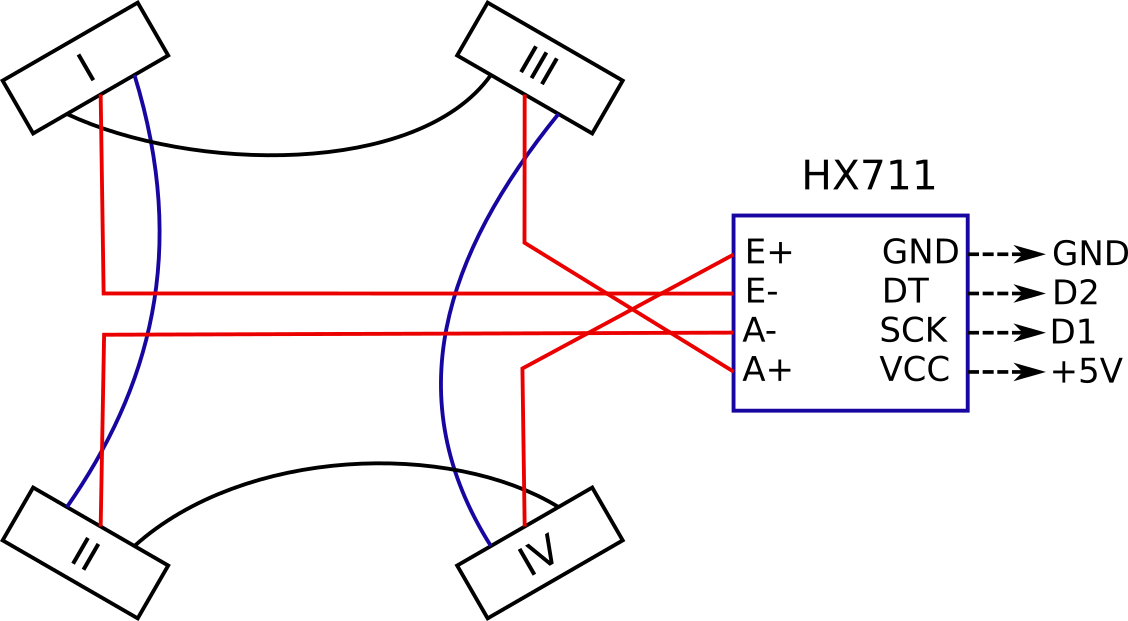
\includegraphics[width=0.65\textwidth]{latex/img/loadcells_scheme.png}
  \caption{The Wheatstone bridge configuration for load cells, connected to the HX711 amplifier; connections from HX711 to NodeMCU board.}\label{img:loadcells_scheme}
\end{figure}


\begin{figure}[!htb]
  \centering
  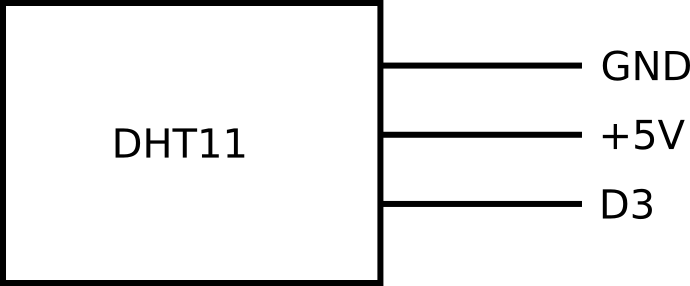
\includegraphics[width=0.4\textwidth]{latex/img/dht_scheme.png}\label{img:dht_scheme}
  \caption{The schematics of DHT11}
\end{figure}

\subsection{Temperature and humidity - DHT11}
A DHT11 sensor is used to get measures of temperature and humidity. The related schematics is in \autoref{img:dht_scheme}.

The library used is \texttt{DHT.h} and the relevant code is \footnote{\url{https://github.com/adafruit/DHT-sensor-library}, \textbf{needs} \url{https://github.com/adafruit/Adafruit_Sensor}}:

\begin{lstlisting}[language=C]
#include "DHT.h"
#define DHTTYPE DHT11
#define DHT11_PIN D3             // signal pin (has to be digital)
DHT dht(DHT11_PIN, DHTTYPE);     // create a DHT11 object
float t = dht.readTemperature(); // read values
float h = dht.readHumidity();
\end{lstlisting}







